\documentclass[11pt]{article}
\usepackage[margin=1in]{geometry}
\usepackage{setspace}
\usepackage{iftex}
\usepackage{amsmath,amssymb}
\usepackage{graphicx}

\ifPDFTeX
  \usepackage[T1]{fontenc}
  \usepackage{newtxtext,newtxmath}
\else
  \usepackage{fontspec}
  \setmainfont{Times New Roman}
\fi

\setstretch{1.0}
\setlength{\parskip}{0.4em}
\setlength{\parindent}{0pt}
\pagenumbering{gobble}

\begin{document}

\begin{titlepage}
\centering
\vspace*{1in}
{\LARGE \textbf{Quantum-Enhanced Strategic Siting of Energy Storage and Microgrids} \par}
\vspace{0.35in}
{\large \textit{Global Industry Challenge (GIC) 2026} \par}
\vspace{0.5in}
{\large Date: \today \par}
\vspace{0.25in}
\centering
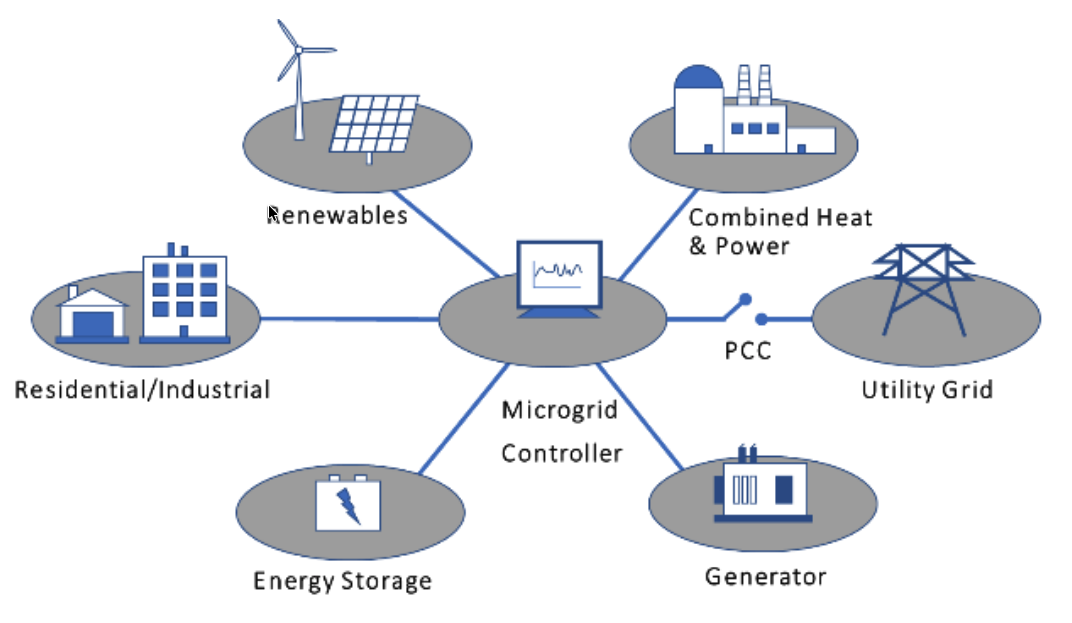
\includegraphics[width=0.80\textwidth]{../../img/microgrid_components.png}
\vspace{0.25em}

{\footnotesize Figure 1: Microgrid architecture and components. Source: S. Atcitty, U.S. Department of Energy presentation.\par}
\vfill
{\large \textbf{Team Name} \par}
\vspace{0.25in}
\begin{tabular}{lll}
Name & Profession \\
\hline
Niraj Venkat & MS/MBA Student and Researcher\\
Muskan Aman  & Electrical Engineer \\
\end{tabular}
\vspace*{0.6in}
\end{titlepage}

\noindent\textbf{Executive Summary}\\
Our project addresses the challenge of resilient, cost-effective deployment of energy storage and microgrids under real grid constraints. The core difficulty is combinatorial: selecting locations, capacities, and operating designs across many scenarios while still honoring AC feasibility and reliability standards. We propose a hybrid workflow where quantum optimization accelerates the discrete planning search and classical solvers enforce physical validity. The framework is explicitly aligned to three outcomes: improved reliability/resilience, reduced lifecycle investment burden, and better operational voltage performance. The output is a ranked set of deployment portfolios with traceable trade-offs and utility-ready feasibility checks.

\noindent\textbf{High-level overview of proposed solution}\\
Our approach uses a Quantum-Assisted Multi-Objective Optimization (QAMOO) loop\footnote{QAMOO reference: Nature Machine Intelligence article, https://www.nature.com/articles/s43588-025-00873-y.} and adapts the multi-objective design used in the Multiverse paper\footnote{Multiverse reference: https://doi.org/10.36227/techrxiv.175502655.52172592/v1.}. A key advantage is that these objectives are already quadratic, so the planning layer is QUBO/Ising-native and avoids quadratization overhead. For binary siting/sizing variables $x_i\in\{0,1\}$, the current surrogate objectives are:
\begin{align*}
C_{\rm R}(x) &= \sum_i \left(\alpha_i x_i^2 + \beta_i x_i + \gamma_i\right), \\
C_{\rm I}(x) &= \sum_i \left(\eta_i x_i^2 + \theta_i x_i + \kappa_i\right), \\
C_{\rm VC}(x) &= x^{\top}Q_{\rm VC}x + q_{\rm VC}^{\top}x + c.
\end{align*}
Here, $C_{\rm R}$ captures resilience/reliability penalty, $C_{\rm I}$ captures capital investment behavior (including economies of scale), and $C_{\rm VC}$ captures voltage-control quality. QAMOO then explores the Pareto front directly across these competing objectives rather than forcing a single fixed preference.

\noindent\textbf{Technical approach}\\
Each candidate from the quantum loop is passed to classical AC power-flow and operating-feasibility checks (thermal limits, voltage bounds, and contingency screens). Infeasible candidates generate cuts and penalties for the next iteration; feasible candidates are retained as Pareto-efficient planning options. Qiskit's \verb|qiskit_addon_opt_mapper| is used for Hamiltonian construction, parameterized-circuit execution, and shot-based sampling, while classical solvers handle power-flow validation and scenario evaluation. Currently we exploit the simpler quadratic form for efficient QUBO execution; in follow-on work, Qiskit can ingest higher-order (HUBO) formulations when richer objectives are needed.

\noindent\textbf{Projected industry impact}\\
For energy stakeholders, this architecture provides a practical path to decision support at planning scale, not just an isolated quantum demo. First, utilities gain faster exploration of resilient infrastructure portfolios when outage and uncertainty dimensions are large. Second, planners receive transparent trade-offs between resilience, investment, and operational performance in a form compatible with existing integrated resource and distribution planning workflows. Third, the hybrid design preserves trust: every quantum-suggested portfolio is filtered through classical validation before recommendation.

The long-term impact is a repeatable method for accelerating grid modernization decisions with measurable reliability and cost benefits.

\end{document}
